% TEMPLATE for Usenix papers, specifically to meet requirements of
%  USENIX '05
% originally a template for producing IEEE-format articles using LaTeX.
%   written by Matthew Ward, CS Department, Worcester Polytechnic Institute.
% adapted by David Beazley for his excellent SWIG paper in Proceedings,
%   Tcl 96
% turned into a smartass generic template by De Clarke, with thanks to
%   both the above pioneers
% use at your own risk.  Complaints to /dev/null.
% make it two column with no page numbering, default is 10 point

% Munged by Fred Douglis <douglis@research.att.com> 10/97 to separate
% the .sty file from the LaTeX source template, so that people can
% more easily include the .sty file into an existing document.  Also
% changed to more closely follow the style guidelines as represented
% by the Word sample file.

% Note that since 2010, USENIX does not require endnotes. If you want
% foot of page notes, don't include the endnotes package in the
% usepackage command, below.

\documentclass[letterpaper,twocolumn,10pt]{article}
\usepackage{usenix,epsfig,endnotes,parskip,amsmath,amssymb,stfloats,placeins,capt-of,subfiles,color,latexsym,ifthen}

\begin{document}

\title{\Large \bf A Protocol for Interledger Payments}

\author{
\textnormal{Stefan Thomas \& Evan Schwartz} \\
\textnormal{\texttt{\{stefan,evan\}@ripple.com}}
}

\maketitle

\thispagestyle{empty}
\section*{Abstract}

We present a protocol for payments across payment systems. It enables secure transfers between \textit{ledgers} and allows anyone with accounts on two ledgers to create a connection between them. Ledger-provided escrow removes the need to trust these \textit{connectors}. Connections can be composed to enable payments between any ledgers, creating a global graph of liquidity or \mbox{\textit{Interledger}}.

Unlike previous approaches, this protocol requires no global coordinating system or blockchain. Transfers are escrowed in series from the sender to the recipient and executed using one of two modes. In the \textit{Atomic} mode, transfers are coordinated using an ad-hoc group of \textit{notaries} selected by the participants. In the \textit{Universal} mode, there is no external coordination. Instead, bounded execution windows, participant incentives and a \mbox{``reverse''} execution order enable secure payments between parties without shared trust in any system or institution.


\section{Introduction}

Sending money today within any single payment system is relatively simple, fast and inexpensive. However, moving money between systems is cumbersome, slow and costly, if it is possible at all.

Digital payment systems use \textit{ledgers} to track accounts and balances and to enable local transfers between their users. Today, there are few \textit{connectors} facilitating payments between these ledgers and there are high barriers to entry for creating new connections. Connectors are not standardized and they must be trusted not to steal the sender's money.

In this paper, we present a protocol for \mbox{\textit{interledger}} payments that enables anyone with accounts on two ledgers to create connections between them. It uses ledger-provided \textit{escrow}---conditional locking of funds---to allow secure payments through untrusted connectors.

Any ledger can integrate this protocol simply by enabling escrowed transfers.
Unlike previous approaches, our protocol does not rely on any global coordinating system or ledger for processing payments---centralized \cite{davies1989security} or decentralized \cite{mazieresstellar,Bitcoin,schwartz2014ripple}.

Our protocol lowers the barriers to facilitating interledger payments. Connectors compete to provide the best rates and speed. The protocol can scale to handle unlimited payment volume, simply by adding more connectors and ledgers. Composing connectors into chains enables payments between any ledgers and give small or new payment systems the same network effects as the most established systems. This can make every item of value spendable anywhere---from currencies to commodities, computing resources and social credit.

Our protocol provides:
\begin{itemize}
\item Secure payments through any connector using ledger-provided escrow.
\item The sender of a payment is guaranteed a cryptographically signed receipt from the recipient, if the payment succeeds, or else the return of their escrowed funds.
\item Two modes of executing payments: In the \textit{Atomic} mode, transfers are coordinated by an ad-hoc group of \textit{notaries} selected by the participants to ensure all transfers either execute or abort. The \textit{Universal} mode instead uses bounded execution windows and incentives to remove the need for any mutually trusted system or institution.
\end{itemize}

\newpage

The following sections describe our protocol in greater depth. Section \ref{sec:model} introduces the core concepts of the protocol, including the actors involved and the need for ledger-provided escrow. Section \ref{sec:atomic} presents the \textit{Atomic} mode. Section \ref{sec:universal} presents the \textit{Universal} mode. Sequence diagrams and the formal protocol specifications can be found in the Appendix.


\section{Interledger Payments}
\label{sec:model}

A \textit{ledger} may be used to track anything of value---from currency or stocks to physical goods and titles---and may be centralized or decentralized \cite{Bitcoin}. As illustrated in Figure \ref{fig:three-bells}, payments between accounts in the same system are accomplished with a simple \textit{book transfer}.

\begin{figure}[ht]
    \centering
    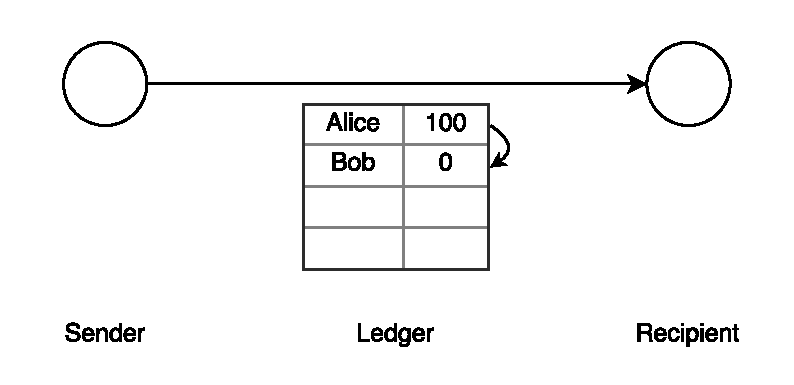
\includegraphics[width=\columnwidth]{figures/three-bells.pdf}
    \caption{Book transfer}
    \label{fig:three-bells}
\end{figure}

A \textit{connector} is a system that facilitates interledger payments by coordinating book transfers on multiple ledgers. Connectors can also translate between different protocols used by these ledgers. As illustrated in Figure \ref{fig:connector}, connector \textit{Chloe} accepts a transfer into her account on one ledger in exchange for a transfer out of her account on another ledger.

\begin{figure}[ht]
    \centering
    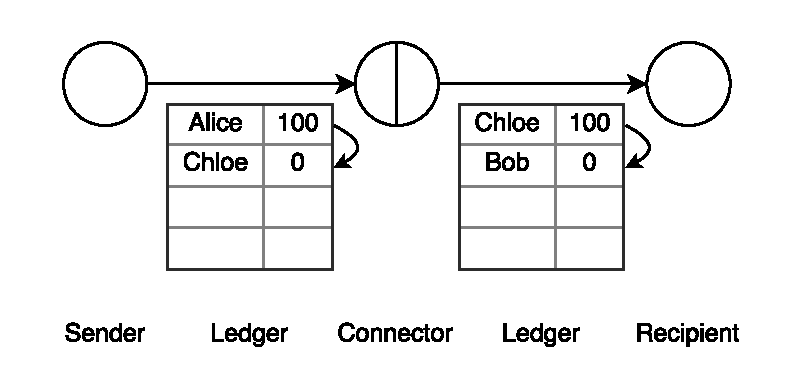
\includegraphics[width=\columnwidth]{figures/connector.pdf}
    \caption{Connector controls accounts on two ledgers}
    \label{fig:connector}
\end{figure}

The problem with existing payment protocols is that the sender must trust the connector to follow through on paying the intended recipient. Nothing technically prevents connectors from losing or stealing money, so they must be bound by reputation and legal contracts to complete the payment correctly. This severely limits the set of institutions that can act as connectors, resulting in a highly uncompetitive and disconnected global payment system.

Ledger-provided escrow guarantees the sender that their funds will only be transferred to the connector once the ledger receives proof that the recipient has been paid. Escrow also assures the connector that they will receive the sender's funds once they complete their end of the agreement.

\begin{figure}[ht]
    \centering
    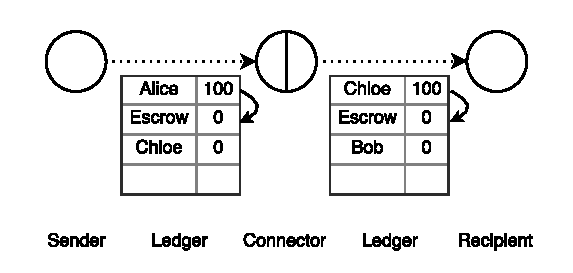
\includegraphics[width=\columnwidth]{figures/connector-escrow.pdf}
    \caption{Funds are escrowed by the sender and connector on their respective ledgers}
    \label{fig:connector-escrow}
\end{figure}

\begin{figure}[ht]
    \centering
    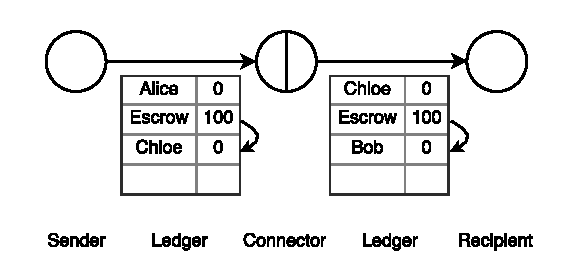
\includegraphics[width=\columnwidth]{figures/connector-execution.pdf}
    \caption{The transfers to the connector and recipient are either executed or aborted together}
    \label{fig:connector-execution}
\end{figure}

The simple arrangement illustrated here can be extended into arbitrarily long chains of connectors to facilitate payments between any sender and any recipient. This brings the small-world network effect (commonly known as the ``six degrees of separation'') \cite{albert1999internet,watts1998collective} to payments and creates a global graph of liquidity or \mbox{\textit{Interledger}}.

\subsection{Byzantine and Rational Actors}

A truly open protocol for payments cannot rely on highly trusted actors for security. It must lower the barriers to participation through built-in protections against potentially faulty, self-interested, or malicious behavior by the participants.

We use the Byzantine, Altruistic, Rational (BAR) model introduced by \cite{aiyer2005bar} for categorizing participants. \textit{Byzantine} actors may deviate from the protocol for any reason, ranging from technical failure to deliberate attempts to harm other parties or simply impede the protocol. \textit{Altruistic} actors follow the protocol exactly. \textit{Rational} actors are self-interested and will follow or deviate from the protocol to maximize their short and long-term benefits.

We assume all actors in the payment are either Rational or Byzantine. Protocols that rely on highly trusted actors effectively assume all to be Altruistic---or bound by factors external to the protocol. Assuming the actors to be self-interested or malicious requires the protocol to provide security even when participants are bound only by the algorithm itself.

We assume that, as Rational actors, ledgers and connectors may require some fee to incentivize their participation in a payment. These fees may be paid in the flow of the payment, or out of band. In this paper, we will only discuss the details of fees necessary to mitigate risks and attacks specific to interledger payments.

While ledgers may be Byzantine, we do not attempt to introduce fault-tolerance---protection against accidental or malicious errors---for participants who hold accounts with such a ledger. Ledgers themselves can be made Byzantine fault-tolerant \cite{mazieresstellar,Bitcoin,schwartz2014ripple}, and participants can choose the ledgers with which they hold accounts. We only seek to isolate participants who hold accounts on non-faulty ledgers from risk.

We assume that connectors will agree to participate in a payment only if they face negligible or manageable risk for doing so, and that they will charge fees accordingly. Connectors will only deliver money on a destination ledger if doing so benefits them directly.

Any of the participants in a payment may attempt to overload or defraud any of the other actors involved. Thus, escrow is needed to make secure interledger payments.


\subsection{Cryptographic Escrow}

Ledger-provided escrow enables secure interledger payments by isolating each participant from the risks of failure or malicious behavior by others involved in the payment. It represents the financial equivalent of the states in the Two-Phase Commit Protocol \cite{Gray:1978:NDB:647433.723863,gray2006consensus}.

Providing escrowed transfers is the main requirement for ledgers to enable secure interledger payments.

All participants rely upon their ledgers to escrow funds and release them only when a predefined condition is met. The sender is assured by their ledger that their funds are transferred only upon delivery of a non-repudiable acknowledgement that the recipient has received their payment. The recipient is assured by their ledger that they will be paid when they provide such an acknowledgement. Connectors also use their ledgers' escrow to protect themselves from risk.

Cryptographic signatures are a simple way for ledgers to securely validate the outcome of the external conditions upon which a transfer is escrowed. Any one-way function can be used \cite{rompel1990one}. Using asymmetric cryptography, the ledger escrows funds pending the presentation of a valid signature for a pre-defined public key and message or hash. The ledger can then easily validate the signature when it is presented and determine if the condition has been met.

\begin{figure}[ht]
    \centering
    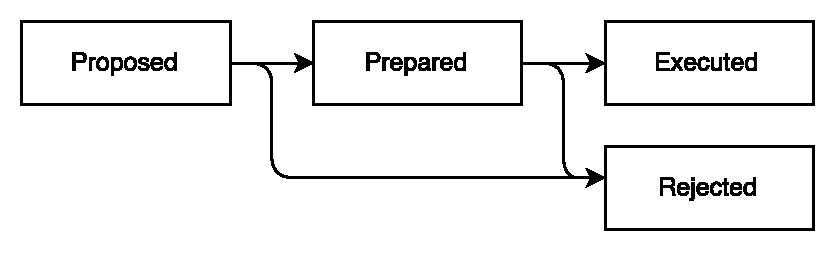
\includegraphics[width=\columnwidth]{figures/transfer-states.pdf}
    \caption{Transfer states}
    \label{fig:transfer-states}
\end{figure}

Figure \ref{fig:transfer-states} illustrates the states of a transfer. First, a transfer is \textit{proposed} to the participants, but no changes are made to the ledger. Once affected account holders have authorized the transfer, the ledger checks that funds are available and that all of its rules and policies have been satisfied. The ledger places the funds in escrow and the transfer is \textit{prepared}. If the execution condition $e$ is fulfilled, the transfer is \textit{executed}. If any of the checks fail, or if an abort condition $e'$ is fulfilled, the transfer is \textit{aborted} and the escrowed funds are returned to their originator.

\section{Atomic Interledger Payments}
\label{sec:atomic}

\begin{figure*}[th!]
    \centering
    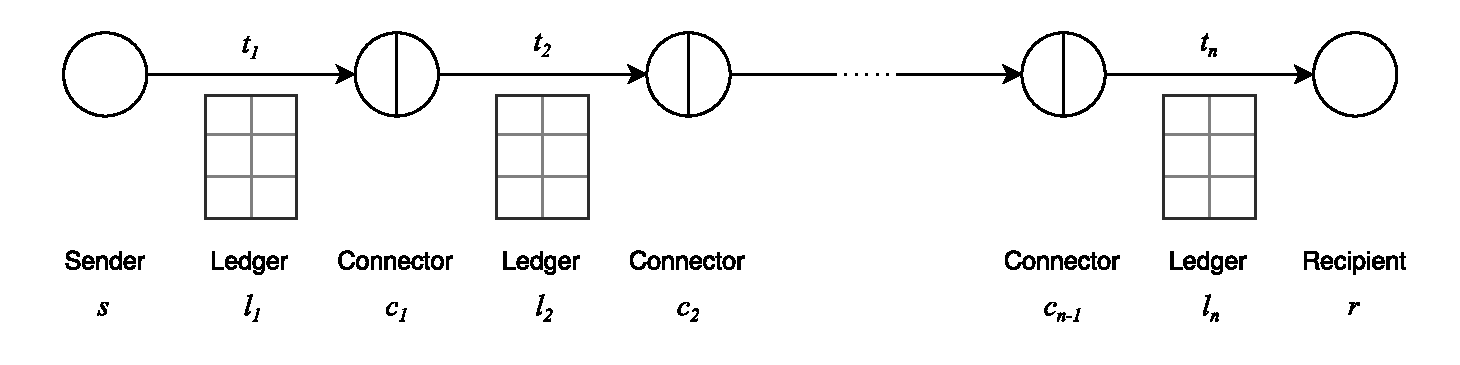
\includegraphics[width=\textwidth]{figures/payment-chain.pdf}
    \caption{Payment chain}
    \label{fig:n-bells}
\end{figure*}

Interledger payments consist of transfers on different ledgers. If the payment partially executes, at least one of the participants loses money. Thus, participants want \textit{atomicity}---a guarantee that all of the component transfers will either execute or that all will be aborted.

Executing transfers atomically across multiple ledgers requires a \textit{transaction commit protocol}. The simplest such protocol is the Two-Phase Commit, in which all systems involved first indicate their readiness to complete the transaction, and then execute or abort based on whether all of the other systems have agreed. The basic form of that protocol uses a \textit{transaction manager} to collect the responses of the various system and disseminate the decision. Fault tolerance can be added to the Two-Phase Commit by replacing the single transaction manager with a group of coordinators that use a consensus algorithm to agree on the outcome of the payment \cite{gray2006consensus}.

The Atomic execution mode uses a Byzantine fault-tolerant agreement algorithm amongst an ad-hoc group of coordinators or \textit{notaries} to synchronize the execution of the component transfers. Additionally, it guarantees that the sender receive a cryptographically signed payment receipt from the recipient if funds are transferred.

Figure \ref{fig:n-bells} shows a payment through a chain of participants $P$ and ledgers $L$. There are $n$ participants in $P$, such that $ \left\vert{P}\right\vert = n $. The sender is the first participant $p_1$ and the recipient is the last participant $p_n$. The connectors $C$ are participants $p_2$ through $p_{n-1}$, such that $ \{ p_i \in C \mid C \subset P \land i \in \mathbb{Z}^+ \land 1 < i < n \} $. The payment consists of $n-1$ book transfers $B$ on $n-1$ ledgers, such that $\left\vert{B}\right\vert = \left\vert{L}\right\vert = n-1 $. The first participant, the sender $p_1$, has an account on ledger $\ell_1$. The last participant, the recipient $p_n$, has an account on ledger $\ell_{n-1}$. Each connector $p_i \in C$ has accounts on ledgers $\ell_{i-1}$ and $\ell_i$ and facilitates payments between them.


\subsection{Notaries}

In the Atomic mode, transfers are coordinated by a group of \textit{notaries} $N$ that serve as the source of truth regarding the success or failure of the payment. They take the place of the transaction manager in a basic Two-Phase Commit. Importantly, notaries are organized in ad-hoc groups for each payment and our protocol does not require one globally trusted set of notaries.

All of the escrow conditions for the book transfers $B$ comprising the payment must depend on the notaries either sending a \textit{D\_Execute} or \textit{D\_Abort} message. If the escrow conditions were based solely on a message from $N$, however, faulty notaries could cause the transfers to execute before the final transfer to the recipient is \textit{L\_Prepared}. \cite{dolev1983authenticated}.

Notaries $N$ must only agree on the \textit{D\_Execute} or \textit{D\_Abort} messages if they have received a signed receipt, the \textit{R\_ReceiptSignature}, from the recipient $p_n$ before a timeout $t$. The recipient's signature provides non-repudiable proof that they have been paid. The recipient $p_n$ signs the receipt once the transfer into their account is \textit{L\_Prepared} and escrowed pending their signature.

To ensure all of the transfers $B$ can be executed atomically, all of the execution conditions $E$ must depend on the \textit{D\_Execute} message from the notaries and the \textit{R\_ReceiptSignature} from the recipient:

\begin{equation}
\forall e \in E : e = \textit{R\_ReceiptSignature} \land \textit{D\_Execute}
\end{equation}

The abort conditions $E'$ for each transfer in $B$ are dependent only on the abort message \textit{D\_Abort}. Receipt of a message fulfilling the abort condition $e'_i$ where $\{ i \in \mathbb{Z}^+ \land i < n \}$ causes the ledger $\ell_i$ to immediately transition the \textit{L\_Proposed} or \textit{L\_Prepared} transfer $b_i$ to the \textit{L\_Aborted} state and release the funds to the originator.

\begin{equation}
\forall e' \in E' : e' = \textit{D\_Abort}
\end{equation}


\subsection{Fault Tolerance}
\label{subsec:fault-tolerance}

The Atomic mode only guarantees atomicity when notaries $N$ act honestly. Like all other participants, we assume notaries are either rational or Byzantine. Rational actors can be incentivized to participate with a fee.

Byzantine notaries, however, could sign both \textit{D\_Execute} and \textit{D\_Abort} messages, communicate them to different ledgers and cause some transfers to be executed and other to be aborted. In order to protect against this, we must set a fault-tolerance threshold $f$. This means that the outcome of the agreement protocol will be correct so long as there are no more than $f$ Byzantine notaries in $N$.

If $f = 0$, we only need a single notary $N = \{ N_1 \}$ and the \textit{D\_Execute} and \textit{D\_Abort} messages are simply signatures by that notary $N_1$.

If $f \geq 1$, notaries use a Byzantine fault-tolerant (BFT) agreement protocol. Using the method from \cite{gray2006consensus,mohan1983method}, a BFT replication algorithm, such as PBFT \cite{castro1999practical} or Tangaroa, a BFT version of Raft \cite{copelandtangaroa}, can be simplified into a binary agreement protocol.

The minimum number of processes required to tolerate $f$ Byzantine faults is $\left\vert{N}\right\vert = 3f + 1$ as shown by \cite{bracha1985asynchronous}.

The \textit{D\_Execute} and \textit{D\_Abort} messages are collections of signatures from some representative subset $N_{rep}$ such that $N_{rep} \subseteq N$ and $|N_{rep}| = f+1$ vouching for the outcome of the agreement protocol.


\subsection{Timeout}
\label{subsec:timeout}

To ensure that funds cannot be held in escrow forever, even in the case of failure, notaries $N$ enforce a timeout $t$. The recipient $p_n$ must submit the \textit{R\_ReceiptSignature} to the notaries $N$ before $t$ is reached, or the payment will be aborted and the escrowed funds returned. $t$ must be sufficient to account for the duration of the phases of the protocol leading up to Execution.


\subsection{Phases of the Protocol}

Before a payment can occur, the sender $p_1$ must find a suitable set of connectors $C$ forming a path to the recipient $p_n$. Connectors have an interest in making their liquidity information available in order to attract payment flows. The problems of minimum-cost and multicommodity flow have been studied extensively in the context of planning \cite{ahuja1988network,cai2001time,wagner1959class}.

In the following, we assume that a path has already been chosen and the exchange rates and any fees quoted by the connectors in $C$ are known.

Appendix \ref{sec:atomic-sequence} illustrates the phases of the protocol, excluding Notary Selection and Notary Setup.


\subsubsection{Notary Selection}
\label{subsec:notary-selection}

Notaries are selected by the participants $P$.

For each candidate fault tolerance threshold $f_c$ where $f_c \in Z^+ \land f_c < f_{max}$ and $f_{max}$ is the sender's maximum fault tolerance threshold, the sender requests the set of all notaries trusted at the given fault tolerance threshold $f_c$ from each participant $p$, $N_p(f_c)$ and calculates the candidate set $N_c(f_c)$ at threshold $f_c$ as the intersection of these sets. Each $p \in P$ chooses $N_p(f_c)$ such that they believe that there is no Byzantine subset $N_{evil}$ where $N_{evil} \subseteq N_p(f_c), |N_{evil}| > f$ which will collude against them.

\begin{equation}
\forall f_c \in Z^+ \land f_c < f_{max} : N_c(f_c) = \bigcap_{p \in P} N_p(f_c)
\end{equation}

Finally the sender chooses a fault tolerance threshold $f$ and a corresponding set of notaries $N$ such that $N \subseteq N_c(f) \land \left\vert{N}\right\vert \geq 3f+1$. If no such set exists, the sender cannot rely on the Atomic mode and must instead use the Universal mode as described in Section \ref{sec:universal}.


\subsubsection{Proposal}

In the proposal phase, the sender $p_1$ notifies each connector $ \{ p_i \mid i \in \mathbb{Z}^+ \land 1 < i < n \} $ about the the book transfers $b_{i-1}$ and $b_i$ in the upcoming payment. Upon receiving the proposal, each connector $p_i$ will verify the proposed spread between the payments matches its exchange rate, charge its fee and store the payment details. $p_i$ accepts the terms of the book transfers $b_{i-1}$ and $b_i$ and the sender $p_1$ proceeds to the next phase.


\subsubsection{Preparation}

Unlike in a basic Two-Phase Commit, book transfers
$ \{ b_i \in B \mid i \in \mathbb{Z}^+ \land 1 < i < n \} $
are prepared in sequence from $b_1$ to $b_{n-1}$. Each connector is only willing to escrow their funds if they know funds have already been escrowed for them.

The sender $p_1$ first authorizes and sends the instruction to prepare the first transfer $b_1$ on $\ell_1$. $p_1$ then requests that the first connector $p_2$ prepare $b_2$ on $\ell_2$. The connector $p_2$ is comfortable preparing $b_2$ because $b_1$ is prepared and the funds have been escrowed by $\ell_1$. Similarly, each connector $p_i$ prepares transfer $b_i$ once it is notified that $\ell_{i-1}$ has prepared $b_{i-1}$ and escrowed the corresponding funds.


\subsubsection{Execution}

Once the last book transfer $b_{n-1}$ has been prepared and the funds escrowed, the recipient $p_n$ must sign the receipt before the timeout $t$. $p_n$ is comfortable signing the receipt because they know that doing so will fulfill the condition of the escrowed funds waiting for them on $\ell_{n-1}$. $p_n$ submits the \textit{R\_ReceiptSignature} to the notaries $N$, who then run the agreement protocol (see Section \ref{subsec:fault-tolerance}) to decide whether the payment should execute.

If $N$ agree that the \textit{R\_ReceiptSignature} was received in time, they submit it and a signed \textit{D\_Execute} message to all participants $P$. Each participant $ \{ p_i \in P \mid i \in \mathbb{Z}^+ \land 1 < i \leq n \} $ submits the \textit{R\_ReceiptSignature} and \textit{D\_Execute} message to $\ell_{i-1}$ to execute $b_{i-1}$ and claim the funds they are due.

If $N$ agree that the payment timed out, they submit a signed \textit{D\_Abort} message to $P$. Each participant $ \{ p_j \in P \mid j \in \mathbb{Z}^+ \land 1 \geq j < n \} $ submits the \textit{D\_Abort} message to $\ell_j$ and reclaims its escrowed funds.


\subsection{Correctness}

The Atomic mode of the protocol inherits the assumptions and level of fault-tolerance from the Byzantine agreement protocol used amongst the notaries. For the purpose of this section, we assume the notaries use PBFT \cite{castro1999practical}.

Given the assumptions in \cite{castro1999practical} we require no additional assumptions.


\subsubsection{Safety}

Safety means that if one non-faulty ledger transitions its transfer to the \textit{L\_Executed} state, then no non-faulty ledger will transition a transfer belonging to the same payment to the \textit{L\_Aborted} state and vice versa. If liveness also holds, all transfers will eventually be executed or all aborted.

Given the safety of the consensus algorithm used by the notaries,
% TODO add citation
we know that all ledgers will only receive one of either: $f + 1$ \textit{D\_Execute}, or $f + 1$ \textit{D\_Abort} messages from notaries. A correct ledger only executes the transfer when it has received $f + 1$ \textit{D\_Execute} messages which precludes the possibility that any other correct ledger has aborted their transfer. Equally, a correct ledger only aborts the transfer when it has received $f + 1$ \textit{D\_Abort} messages which precludes the possibility that any other correct ledger has received $f + 1$ \textit{D\_Execute} messages and aborted their transfer.


\subsubsection{Liveness}

Liveness means that every non-faulty ledger connected to at least one non-faulty, rational participant will eventually execute or abort its transfer.

As mentioned in Section \ref{subsec:timeout}, the notaries will initiate their agreement protocol spontaneously after a timeout $t$. From the liveness property of the underlying agreement protocol, we know that the notaries will eventually decide to either \textit{D\_Execute} or \textit{D\_Abort} and broadcast that decision to the participants. Each ledger is connected to at least two participants. If one of these participants is non-faulty, it will forward the decision to the ledger.

Note that if notaries could broadcast directly to the ledgers, our protocol could maintain liveness even when all participants are faulty. However, in real world applications, some ledgers use proprietary protocols or private networks, so we cannot rely on the fact that the notaries can reach them directly.

If a transfer is in the \textit{L\_Prepared} state, at least one of the participants has an interest in seeing the transfer reach a final state, because the escrowed funds would be transferred to them. If this participant is rational they will therefore eventually forward the notaries' decision. A Byzantine participant in this position may not, but in doing so does not hurt anyone else.


\subsection{Fees}
\label{subsec:fees}

Each connector in $C$ incurs some costs and risks for participating in a payment, which can be priced into the connectors' fees.

When trading different assets, connectors in $C$ effectively write the sender $p_1$ an \textit{American option} \cite{black1973pricing,brennan1977valuation}
which, on exercise, swaps an asset on one ledger for an equivalent asset on another ledger.
In addition to the factors considered in standard option pricing, the connector should also account for the following attack in its fee.


\subsubsection{Liquidity Starvation}

An attacker can attempt to temporarily tie up all of a connector's liquidity in payments it knows will fail. This attack is rendered uneconomical if the connector sets its fee to cover its costs and the profit it would expect if the payment were successful. Furthermore, connectors, including those operated by the same entity as a ledger, can prevent their funds from being completely tied up by escalating their fees as a function of the percentage of their total liquidity being held in escrow.

\newpage

\section{Universal Interledger Payments}
\label{sec:universal}

While the Atomic mode uses notaries to ensure proper execution of a payment, the Universal mode relies on the incentives of rational participants instead to eliminate the need for external coordination. It provides safety and liveness for all non-faulty participants connected to only non-faulty ledgers, under an assumption of bounded synchrony with a known bound. In Section \ref{subsubsec:optimal-timeouts} we discuss the practical considerations of using Universal mode in a system that does not guarantee bounded synchrony, e.g. the Internet.

Appendix \ref{sec:universal-sequence} illustrates the phases of the payment in this mode.


\subsection{Execution Order}

In Universal mode, there are no notaries. The book transfers $B$ must be executed in a specific order to ensure all participants' incentives are aligned to execute the payment properly and to ensure delivery of the \textit{R\_ReceiptSignature} to the sender $p_1$.

The transfers $B$ are escrowed only on the condition of receiving the \textit{R\_ReceiptSignature}:

\begin{equation}
\forall e \in E : e = \textit{R\_ReceiptSignature}
\end{equation}

Instead of having a global timeout, each book transfer in $ \{ b_i \in B \mid i \in \mathbb{Z}^+ \land i < n \} $ has its own expiration time enforced by the ledger $\ell_i$.
After the last book transfer $b_{n-1}$ is prepared, the recipient $p_n$ signs the receipt and presents the \textit{R\_ReceiptSignature} directly to their ledger $\ell_{n-1}$. If it is before the transfer's expiration time $t_{n-1}$, $b_{n-1}$ will be executed immediately.

Once $b_{n-1}$ is executed and the recipient $p_n$ is paid, connector $p_{n-1}$ has a very strong incentive to pass the \textit{R\_ReceiptSignature} back to $\ell_{n-2}$, as they have paid out money but have not yet been paid. When each connector $ \{ p_j \in P \mid j \in \mathbb{Z}^+ \land 1 < j < n \} $ learns of the execution of the book transfer $b_j$, they must get the \textit{R\_ReceiptSignature} from $\ell_j$ and submit it to $\ell_{j-1}$ to claim the money waiting in escrow for them.

Thus, the transfers in $B$ are executed in ``backwards'' order, from the recipient $p_n$ to the sender $p_1$. Once the first transfer $b_1$ is executed, the sender $p_1$ can get the \textit{R\_ReceiptSignature} from their ledger $\ell_1$.

If the last transfer $b_{n-1}$ times out before $p_n$ submits the \textit{R\_ReceiptSignature}, all transfers in $B$ will expire and the escrowed funds will be returned to their originator. The following section discusses expiration times and the message delay risk connectors must manage.


\subsection{Message Delay}
\label{subsec:message-delay}

Each book transfer in $B$ must have an expiration time $t$ to ensure liveness. In order for a connector $ \{ p_i \in P \mid i \in \mathbb{Z}^+ \land 1 < i < n \} $ to agree to take part in the payment, they must be able to pass the \textit{R\_ReceiptSignature} from ledger $\ell_i$ to $\ell_{i-1}$ and execute $b_{i-1}$ before it expires. If $b_i$ is executed but $b_{i-1}$ expires, $p_i$ loses money. Because $b_i$ may execute very close to its expiration time $t_i$, the expiration time $t_{i-1}$ for transfer $b_{i-1}$ must be greater than that of $b_i$ by some finite time difference $t_{i-1} - t_i$.

This time difference $t_{i-1} - t_i$ must account for the messaging delays $M(\ell_i, p_i)$ from $\ell_i$ to $p_i$ and $M(p_i, \ell_{i-1})$ from $p_i$ to $\ell_{i-1}$ (which includes the processing delays at $p_i$, $\ell_i$ and $\ell_{i-1}$ respectively) and the clock skew $K(\ell_{i-1}, \ell_i)$ between ledgers $\ell_{i-1}$ and $\ell_i$.

\begin{equation}
\label{eq:expiration-delta}
t_i \geq t_{i+1} + M(\ell_i, p_{i+1}) + M(p_{i+1}, \ell_i) + S(\ell_i, \ell_{i+1})
\end{equation}

The timeout $t_{n-1}$ for the destination transfer $b_{n-1}$ is equal to the timeout $t$ in Atomic mode introduced in Section \ref{subsec:timeout}. That is, it is large enough to allow for the preparation of the transfers and for the recipient to sign and submit the \textit{R\_ReceiptSignature}.


\subsection{Correctness}

For our analysis of Universal mode, we consider both safety and liveness under bounded synchrony. We define bounded synchrony similar to the definition given in \cite{dwork1988consensus} as a system in which there is a known upper bound $M$ on messaging delays between processes and a known upper bound $S$ on clock skew between two nodes. We assume that processing times are negligible and included in $M$.


\subsubsection{Safety}

Safety means that there will be no book transfer $ \{ b_i \in B \mid i \in \mathbb{Z}^+ \land i < n-1 \} $ which expires if $b_{i+1}$ executed unless $\ell_i$, $\ell_{i+1}$ or participant $p_{i+1}$ are faulty.

Let $b_{i+1}$ execute at time $\phi_0$. We know that $b_{i+1}$ was not expired, therefore:

\begin{equation}
\label{eq:phi0}
\phi_0 < t_{i+1}
\end{equation}

A correct ledger $\ell_{i+1}$ will send a message $\tuple{\textit{M\_ExecuteNotify}, \textit{R\_ReceiptSignature}}$ to connector $p_{i+1}$ which will arrive at time $\phi_1$:

\begin{equation}
\label{eq:phi1}
\phi_1 \leq \phi_0 + M(\ell_i, p_{i+1})
\end{equation}

The rational connector $p_{i+1}$ will send a message $\tuple{\textit{M\_ExecuteRequest}, \textit{R\_ReceiptSignature}}$ to ledger $\ell_i$ which will arrive at time $\phi_2$.

\begin{equation}
\label{eq:phi2}
\phi_2 \leq \phi_1 + M(p_{i+1}, \ell_i)
\end{equation}

The correct ledger $\ell_i$ is guaranteed to execute transfer $b_i$ if and only if the message arrives before the timeout $t_i$. However, so far we have expressed all times in terms of $\ell_{i+1}$'s local clock. In order to ensure that $b_i$ is not expired, we must account for clock skew:

\begin{equation}
\label{eq:phi3}
t_i \geq \phi_2 + S(\ell_i, \ell_{i+1})
\end{equation}

From equations (\ref{eq:expiration-delta}), (\ref{eq:phi0}), (\ref{eq:phi1}), (\ref{eq:phi2}) and (\ref{eq:phi3}):

\begin{equation}
\begin{split}
t_i & \geq \phi_2 + S(\ell_i, \ell_{i+1}) \\
    & \geq \phi_1 + M(p_{i+1}, \ell_i) + S(\ell_i, \ell_{i+1}) \\
    & \geq \phi_0 + M(\ell_i, p_{i+1}) + M(p_{i+1}, \ell_i) + S(\ell_i, \ell_{i+1}) \\
    & \geq t_{i+1} + M(\ell_i, p_{i+1}) + M(p_{i+1}, \ell_i) + S(\ell_i, \ell_{i+1})
\end{split}
\end{equation}

Since $\ell_i$ is a correct ledger, it will execute the transfer. A transfer that has been executed on a correct ledger cannot expire, therefore $b_i$ cannot expire.


\subsubsection{Liveness}

Liveness means that eventually each book transfer $ \{ b_i \in B \mid i \in \mathbb{Z}^+ \land i < n \} $ on a non-faulty ledger $\ell_i$ must either be \textit{L\_Executed} or \textit{L\_Aborted}.

All book transfers $b_i$ have a finite expiry time $t_i$. A correct ledger $\ell_i$ will expire transfer $b_i$ at time $t_i$ unless it has already executed.

Therefore after time $t_i$, transfer $b_i$ will be either \textit{L\_Executed} or \textit{L\_Aborted}.


\subsection{Fault and Attack Mitigation}

In Section \ref{subsec:fees} we discussed the connector fee in Atomic mode. In Universal mode, there are additional costs that the connector must take into account:


\subsubsection{Optimal Timeouts}
\label{subsubsec:optimal-timeouts}

In an asynchronous system, message delays and clock skew are unbounded, so a connector $ \{ p_i \in P \mid i \in \mathbb{Z}^+ \land 1 < i < n \} $ may lose the race to forward the \textit{R\_ReceiptSignature} from $\ell_i$ to $\ell_{i-1}$, causing them to lose money.

However, by observing prior performance of the network, $p_i$ can estimate the probability $\Pr(t_{i-1} - t_i \geq M(\ell_i, p_{i+1}) + M(p_{i+1}, \ell_i) + S(\ell_i, \ell_{i+1}))$, calculate the value of the risk to them and include it in their fee.

As $t_{i-1} - t_i$ becomes larger, the risk decreases. However, the expiration time for each transfer $ \{ b_j \in B \mid j \in \mathbb{Z}^+ \land j < i-1 \} $ also increases. Longer expiration times incur higher fees, because funds may be held in escrow for a longer period. The sender $p_1$ will try to choose $t_{i-1} - t_i$ such that the total amount of fees is minimized.


\subsubsection{Robust Messaging}

The other participants may collude in an attempt to defraud a connector. In order to do so, they must interfere with the messaging as mentioned in the previous section to prevent the connector $ \{ p_i \in P \mid i \in \mathbb{Z}^+ \land 1 < i < n \} $ from completing the transfer $b_{i-1}$ thereby profiting at $p_i$'s expense.

The mitigation for this attack varies based on the technical characteristics of each ledger. However, in all cases, it is a type of Denial of Service mitigation. Both connectors and ledgers have an interest in establishing reliable communication.


\subsubsection{Receipt Privacy}

The recipient $p_n$ does not have to transfer any money, but we assume that the act of signing the receipt has some external meaning, such as nullifying an existing asset of the recipient (e.g. an invoice) or creating a new liability.

To claim the funds escrowed for them, the recipient $p_n$ must submit \textit{R\_ReceiptSignature} to $\ell_{n-1}$ before the transfer $b_{n-1}$ is executed. In an asynchronous system, $b_{n-1}$ might timeout while this message is in transit.

In order to guarantee safety for the recipient then, we must introduce another property of ledgers, \textit{ReceiptPrivacy}. A correct ledger that offers \textit{ReceiptPrivacy} does not disclose a $\tuple{\textit{D\_Execute}, \textit{R\_ReceiptSignature}}$ message (or the \textit{R\_ReceiptSignature} contained therein) unless $b_i$ is executed successfully.

If the recipient chooses an honest ledger with \textit{ReceiptPrivacy}, they are not at risk, even in an asynchronous system, because their ledger $\ell_{n-1}$ will disclose \textit{R\_ReceiptSignature} if and only if $b_{n-1}$ executes.


\section{Conclusion}

We have proposed a protocol for secure interledger payments across an arbitrary chain of ledgers and connectors. It uses ledger-provided escrow based on cryptographic conditions to remove the need to trust the connectors.

The Atomic mode of the protocol provides atomicity for payment chains in which the participants can agree upon a group of notaries. The Universal mode uses the incentives of rational actors to enable practical payments between participants that do not all share trust in any institution or system.

Our protocol does not rely on any single system for processing payments, so there is no limit to its scalability. Payments can be as fast and cheap as the constituent ledgers and connectors allow and transaction details are private to their participants. The separation of concerns and the minimal standardization requirements enable continuous optimization and competition between connectors and between ledgers.

Removing the need to trust the connector enables anyone with accounts on two or more ledgers to make connections between them. Connectors can be composed to make payments and the financial system more accessible, competitive and resilient. This enables the creation of a global graph of liquidity or \textit{Interledger}.


{\footnotesize \bibliographystyle{acm}
\bibliography{sample}}


\clearpage
\appendix
\section{Appendix}


\subsection{Atomic Mode Sequence Diagram}
\label{sec:atomic-sequence}

\begin{minipage}{\textwidth}
    \centering
    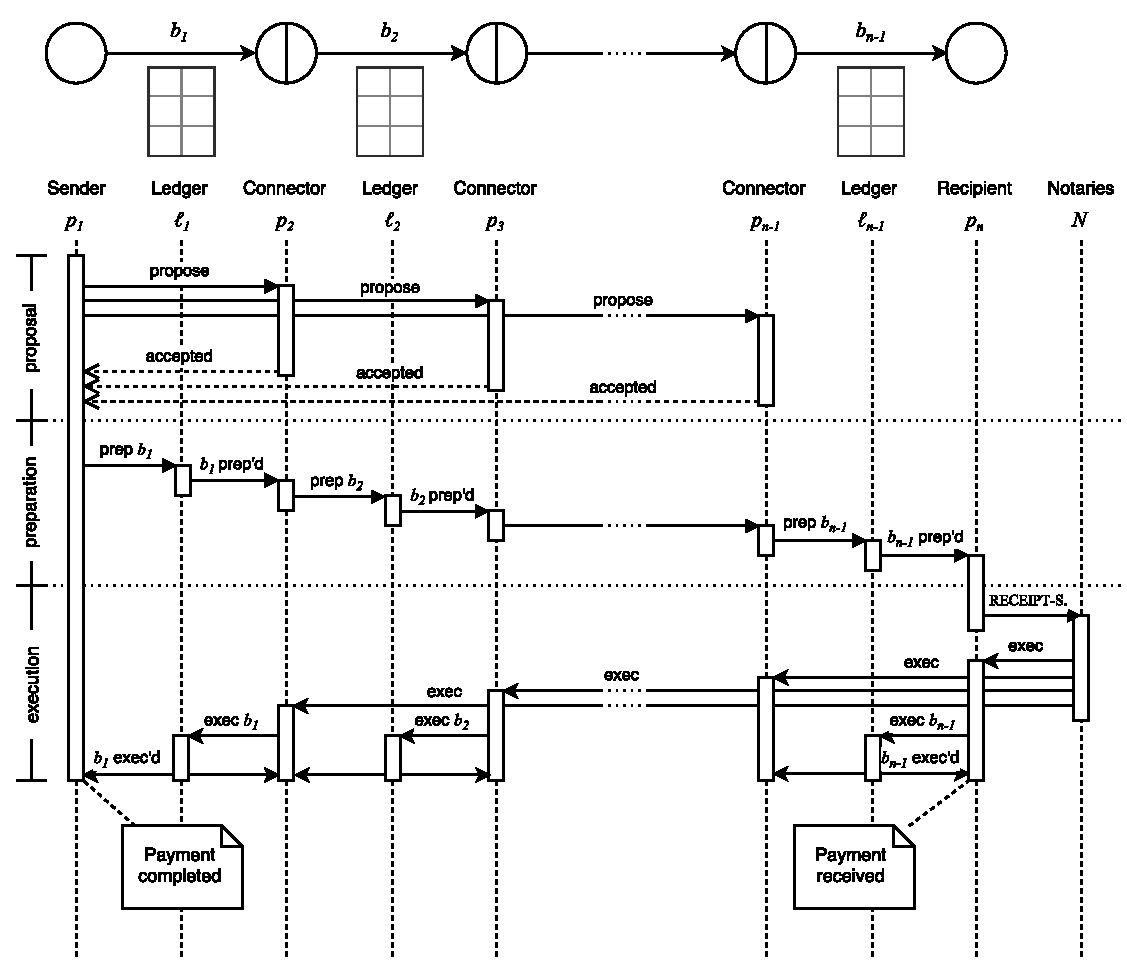
\includegraphics[width=\textwidth]{figures/atomic-sequence.pdf}
    \captionof{figure}{Phases of a payment in the Atomic mode}
\end{minipage}

\clearpage


\subsection{Universal Mode Sequence Diagram}
\label{sec:universal-sequence}

\begin{minipage}{\textwidth}
    \centering
    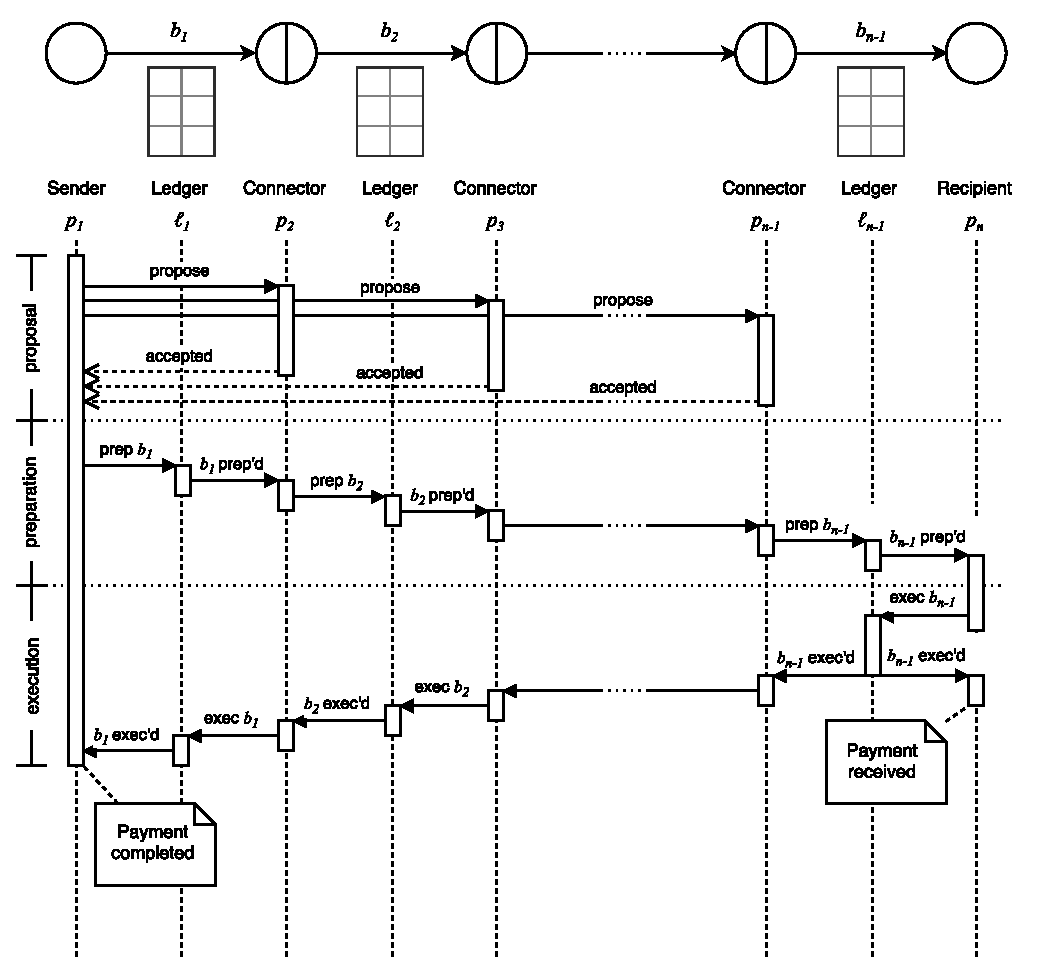
\includegraphics[width=\textwidth]{figures/universal-sequence.pdf}
    \captionof{figure}{Phases of a payment in the Universal mode}
\end{minipage}


\end{document}
